\rule{0.5\textwidth}{0.5pt}\\

	{\large \textbf{Brute Force for HCIPy data}}\\
	
	\paragraph{Data}
	
	There are two groups of datasets.
	\begin{itemize}
		\item The data was generated with Hcipy using an \filename{InfiniteAtmosphericLayer} aberrator.
		\item 4 different datases of PSFs associated to 1 dataset of PL fluxes:
		\begin{itemize}
			\item \textbf{Dataset 1}: Original sized PSF of 128x128 pixels
			\item \textbf{Dataset 2}: Cropped sized PSF of 64x64 pixels (the central pixels of PSFs in Dataset1)
			\item \textbf{Dataset 3}: Original sized predicted PSF from the PL fluxes dataset by a model with 0.0046 train MSE and 0.0560 validation MSE. The model is called PSFReconstructorSuperBig.
			\item \textbf{Dataset 4}: Cropped sized predicted PSF from the PL fluxes dataset by a model with 0.0085 train MSE and 0.2097 validation MSE. The model is called CroppedBNFC.
		\end{itemize}
	\end{itemize}
	
	\paragraph{Dataset shapes}
	\begin{itemize}
		\item \textbf{PSF datasets}: $70000x32768$ 
		\item \textbf{PL intensities}: $70000x19$
	\end{itemize}
	
	The PSF datasets are originally a $128\times128\times2$ matrix with real and imaginary values separated, this matrix is then flattened to compute euclidean distance.
	
	\paragraph{Results}
	
	\begin{figure*}[ht!]
		\centering
		\subfloat[Euclidean distance cloud]{%
		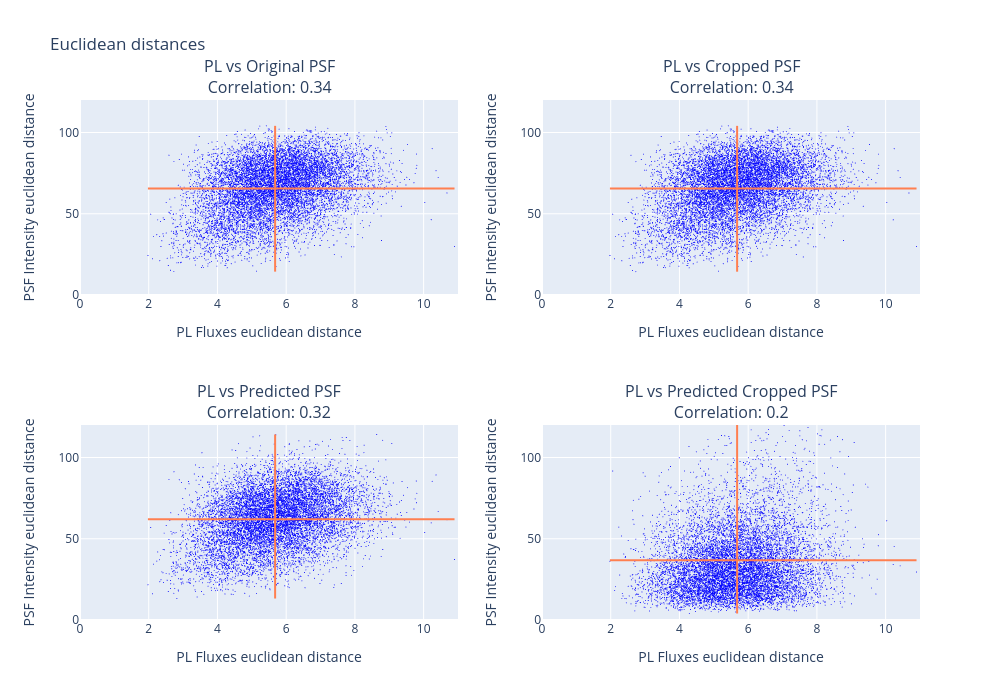
\includegraphics[width=0.7\textwidth]{euclidean_distances.png}}\\
		\subfloat[Euclidean distance ratios]{%
		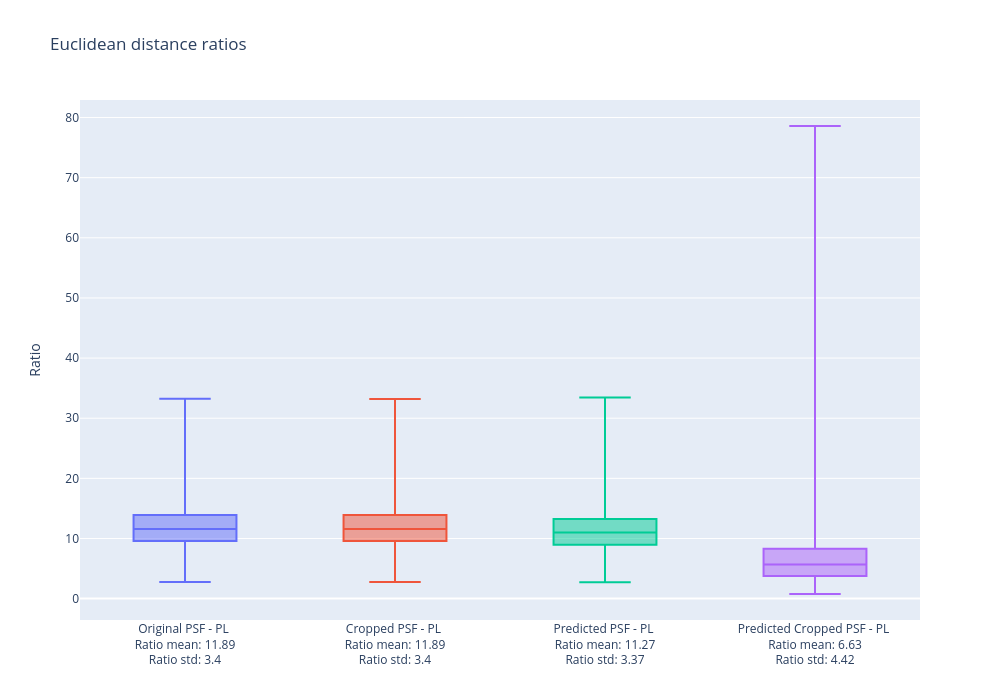
\includegraphics[width=0.7\textwidth]{euclidean_distance_ratios.png}}
		\caption{Euclidean distances ratios between PL and PSF pairs}\hspace{\fill}
	\end{figure*}
	
\FloatBarrier	
\rule{0.5\textwidth}{0.5pt}\\